\documentclass[border=10pt,tikz]{standalone}
\usepackage{tikz}
\usetikzlibrary{positioning,arrows.meta,shapes}
\begin{document}
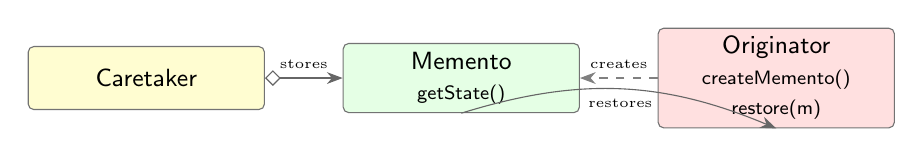
\begin{tikzpicture}[
  font=\sffamily\small,
  cls/.style={rectangle, rounded corners=2pt, draw=black!55, line width=0.4pt,
              minimum height=8mm, minimum width=30mm, inner sep=3pt, fill=white, align=center},
  con/.style={cls, fill=red!12},
  imp/.style={cls, fill=green!10},
  cli/.style={cls, fill=yellow!18},
  agg/.style={{Diamond[length=2mm,width=2mm,open]}-{Stealth[length=2mm]}, draw=black!60},
  arr/.style={-{Stealth[length=2mm]}, draw=black!60},
  ret/.style={-{Stealth[length=2mm]}, dashed, draw=black!50}
]
\node[cli] (ct) at (-4, 0)   {Caretaker};
\node[imp] (m)  at ( 0, 0)   {Memento \\ \scriptsize getState()};
\node[con] (or) at ( 4, 0)   {Originator \\ \scriptsize createMemento() \\ \scriptsize restore(m)};

\draw[agg] (ct.east) -- (m.west) node[midway, above, font=\tiny]{stores};
\draw[ret] (or.west) -- (m.east) node[midway, above, font=\tiny]{creates};
\draw[arr] (m.south) to[bend left=20] node[midway, below, font=\tiny]{restores} (or.south);
\end{tikzpicture}
\end{document}
